\section{Theorie}
\label{sec:Theorie}

\subsection{Grundlagen}
\subsubsection{Vakuum}
Für den Begriff des Vakuums finden sich verschiedenen Definitionen
wie die von Wikipedia \cite[Vakuum ist in der technischen Praxis ein Raum mit weitgehender Abwesenheit von Materie.]{dewiki}.
Normgerecht ist Vakuum definiert als 
\cite[der Zustand eines Gases, 
wenn in einem Behälter der Druck des Gases 
und damit die Teilchenzahldichte niedriger ist als außerhalb oder wenn der Druck des Gases niedriger ist als 300 mbar,
d. h. kleiner als der niedrigste auf der Erdoberfläche vorkommende Atmosphärendruck.]{DIN} 
Fest steht, der Vakuum Begriff hängt mit dem Begriff des Druckes zusammen,
dadurch gibt es nicht das eine Vakuum, sondern vielmehr eine druckabhängige Gliederung,
welche in Abbildung (\ref{fig:Vakuum}) dargestellt ist. 
Zusätzlich sind in der Grafik typische Anwendungen dieser,
sowie Arbeitsbereiche erschiedener Pumpbauweisen aufgelistet.
\begin{figure}[ht]
    \centering
    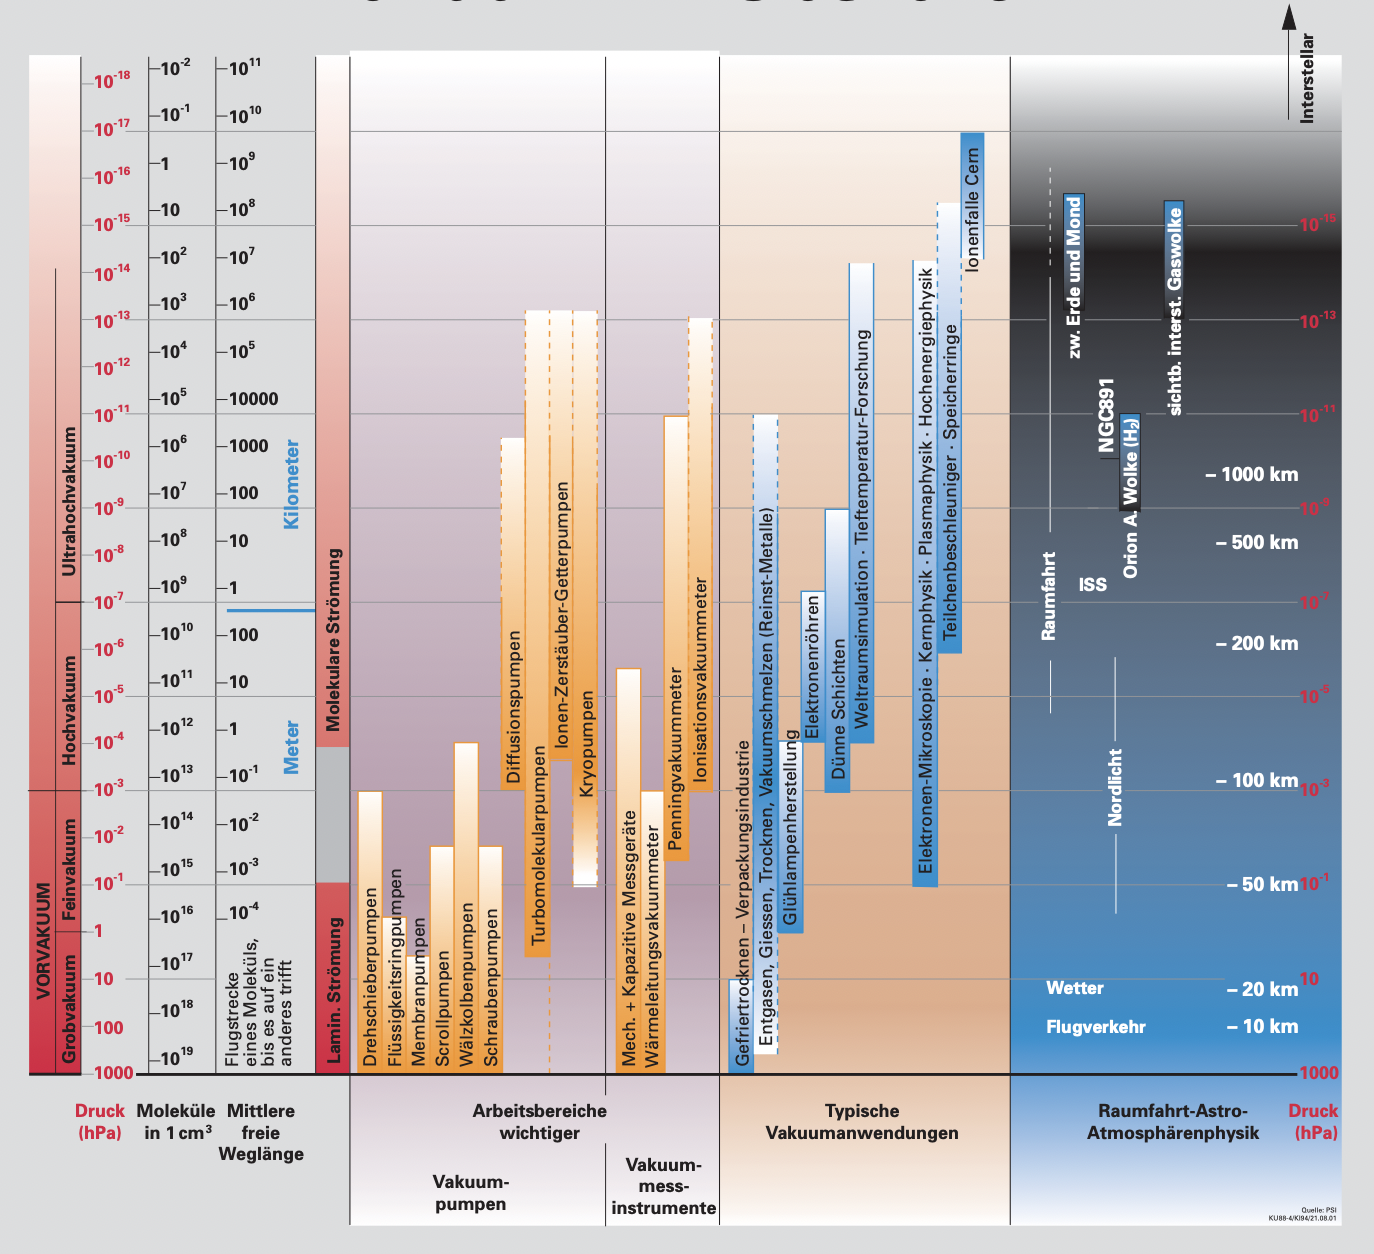
\includegraphics[width=\textwidth]{abb/Vakuum.png}
    \caption{Vakuum im Überblicke \cite{Pfeifer}}
    \label{fig:Vakuum}
\end{figure}

\subsubsection{Druck}
Der Druck ist definiert als die normale Kraft $F$, die auf eine Fläche $A$ wirkt
\begin{equation}
    p = \frac{F}{A}. \label{eq:Druck}
\end{equation}
Der Einfachheit halber gehen wir im folgendem davon aus, 
dass es sich bei den verwendeten Gasen um \textit{Ideale Gase} handelt.
Diese besitzen im Vergleich zu reellen Gasen folgende vereinfachende Eigenschaften:
\begin{itemize}
    \item Ideale Gasteilchen bewegen sich frei und wechselwirken nur durch elastische Stöße
    \item Ideale Gasteilchen punktförmig
    \item Ideale Gasteilchen Vibrieren und Rotieren nicht 
\end{itemize}
Nun lässt sich der Druck als Impulsübertrag zwischen den Gasteilchen und der Fläche $A$ verstehen.  

Viele Gase treten nicht im einheitlichen Zustand auf, sondern als Gemisch.
So ist die Luft größtenteils ein Gemisch aus Stickstoff ($78\%$) und Sauerstoff ($21\%$) \cite{luft}. 
Dafür wird der Partialdruck $p_p$ eingeführt, 
welcher den Druck beschreibt den jede Gaskomponente unabhängig voneinander ausübt.
Die Summe der Partialdrücke ergibt den Totaldruck
\begin{equation}
    p = \sum p_p.
\end{equation}

\subsubsection{Ideale Gasgleichung}
Wichtig zur Untersuchung von Gasen 
und somit auch für den Vakuumversuch sind neben dem \textit{Druck} die Kennzahlen \textit{Volumen} $V$
und \textit{Temperatur} $T$.
Ihr Zusammenhang ist bei idealen Gasen gegeben durch die ideale Gasgleichung
\begin{equation}
    pV=N\cdot k_b\cdot T. \label{eq:idealgaß}
\end{equation}
Dabei steht $k_b$ für die Boltzmann-Konstante. \footnote{$k_b = 1,3806649\cdot10^{-23}$J/K}

\subsubsection{Mittlere freie Weglänge}
Der Fluss und die Ausbreitung von Gasmolekülen wird immer wieder unterbrochen durch Zusammenstöße zwischen den Gasteilchen.
Der mittlere Weg, 
den ein Teilchen zurücklegen kann bevor es mit einem anderen kollidiert, wird die \textit{mittlere freie Weglänge} $\tilde{I}$ genannt.
Sie ist abhängig von der Geschwindigkeit der Teilchen, welche durch die Temperatur beschrieben werden kann,
und der Teilchenzahldichte, welche proportional zum Druck ist.  

\subsubsection{Strömungsarten}
Abhängig von der mittleren freien Weglänge
und der Ausdehnung des Strömungskanals strömen die Gase unterschiedlich durch den Aufbau.
Da $\tilde{I}$ proportional zum Druck ist ändert sich die Strömungsart im besser werdenden Vakuum.

Herrscht im Aufbau ein Grobvakuum kommt es zu vielen Kollisionen zwischen den Teilchen,
aber zu wenigen zwischen Teilchen und Gefäßwand.
Die mittlere freie Weglänge ist deutlich kleiner als die Gefäßabmessungen.
Diese Strömung wird \textit{Visköse Strömung} genannt 
und kann in laminar und turbulent unterteilt werden.
Bei der laminaren Strömung bleiben die Gasteilchen in parallelen Schichten mit verschiedener Geschwindigkeit.
Mit hohen Geschwindigkeiten lösen sich diese Schichten auf, 
sodass von einer turbulenten Strömung gesprochen wird. 
Diese gilt es wenn möglich in der Vakuumtechnik zu vermeiden,
da sie eine höhere Pumpleistung verlangen.

Im Hoch- und Ultrahochvakuum geht die visköse Strömung in eine molekulare Strömung über.
Die mittlere freie Weglänge ist nun deutlich größer als die Ausdehnung der Teilchen,
damit findet so gut wie keine Wechselwirkung zwischen den Gasteilchen statt,
sondern nur noch mit den Gefäßwänden.
Dies wird später besonders für die Turbomolekularpumpe wichtig.
In Abbildung (\ref{fig:strömung}) sind die verschiedenen Strömungsarten modellhaft dargestellt.
\begin{figure}[h]
    \centering
    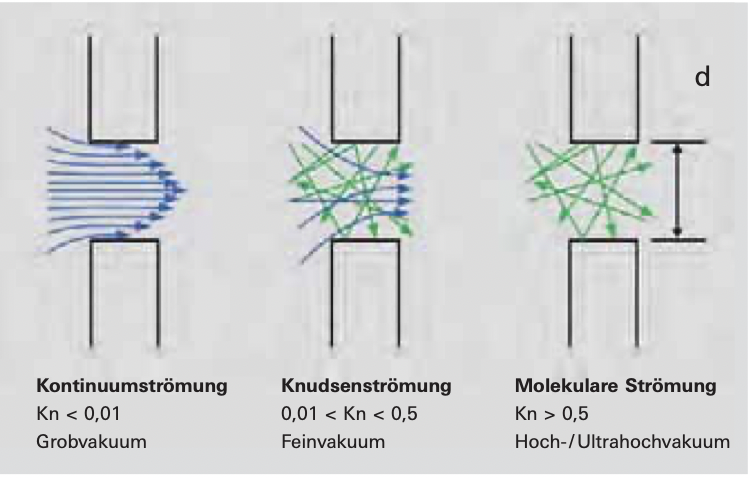
\includegraphics[width=0.5\textwidth]{abb/Stroemungen.png}
    \caption{Profile der Verschiedenen Strömungsarten \cite{Pfeifer}}
    \label{fig:strömung}
\end{figure}

\subsubsection{Leitwert}
In den Röhren zwischen des Rezipienten\footnote{Vakuumkammer} und den Vakuumpumpen kommt es zwischen dem Gas 
und den Wänden zu Reibung, ebenso zwischen den Gasteilchen selbst.
Dies führt zu einem Strömungswiderstand $W$ dessen Kehrwert den Leitwert $L$ bildet
\begin{equation}
    L = \frac{1}{W}.
\end{equation}
Diese Gesetzmäßigkeit ist analog zum ohmschen Widerstand.
Offensichtlich hängt der Leitwert von der vorliegenden Strömungsart ab
und damit in Hinsicht der Vakuumphysik vom Druck.
Dieser Zusammenhang zwischen Druck und Leitwert ist in Abbildung \ref{fig:leitwert} dargestellt.
Es ist zu beobachten, dass gerade für schlechte Vakuume der Leitwert besonders hoch ist,
welches sich in einem Saugleistungsverlust der Pumpen bemerkbar macht.
\begin{figure}[h]
    \centering
    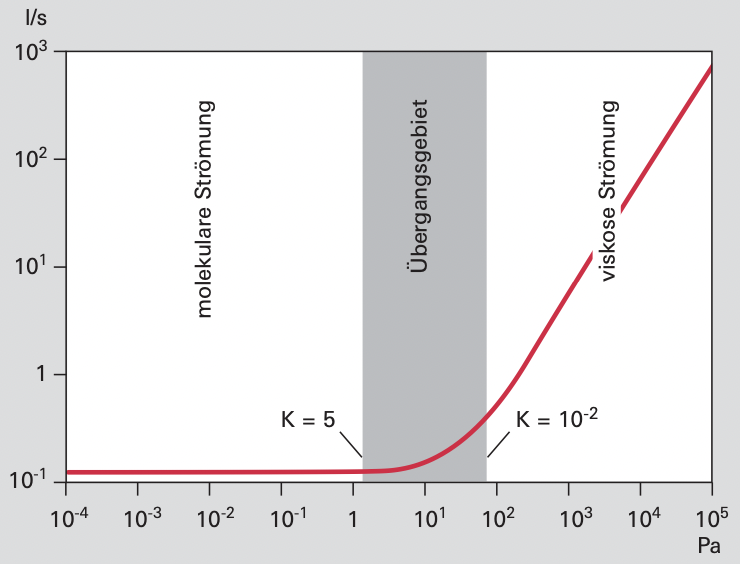
\includegraphics[width=0.7\textwidth]{abb/leitwert.png}
    \caption{Leitwert eines runden glatten Rohrs \cite{Pfeifer}} 
    \label{fig:leitwert}
\end{figure} 



\subsection{Vakuumerzeugung}
\subsubsection{Grundlagen}
Wie in Abbildung \ref{fig:pumpen} zu sehen ist, gibt es eine Vielzahl verschiedener Pumpen,
die sich in drei große Kategorien einteilen lassen:
Verdränger-, kinetische und gasbindende Vakuumpumpen.
\begin{figure}[h]
    \centering
    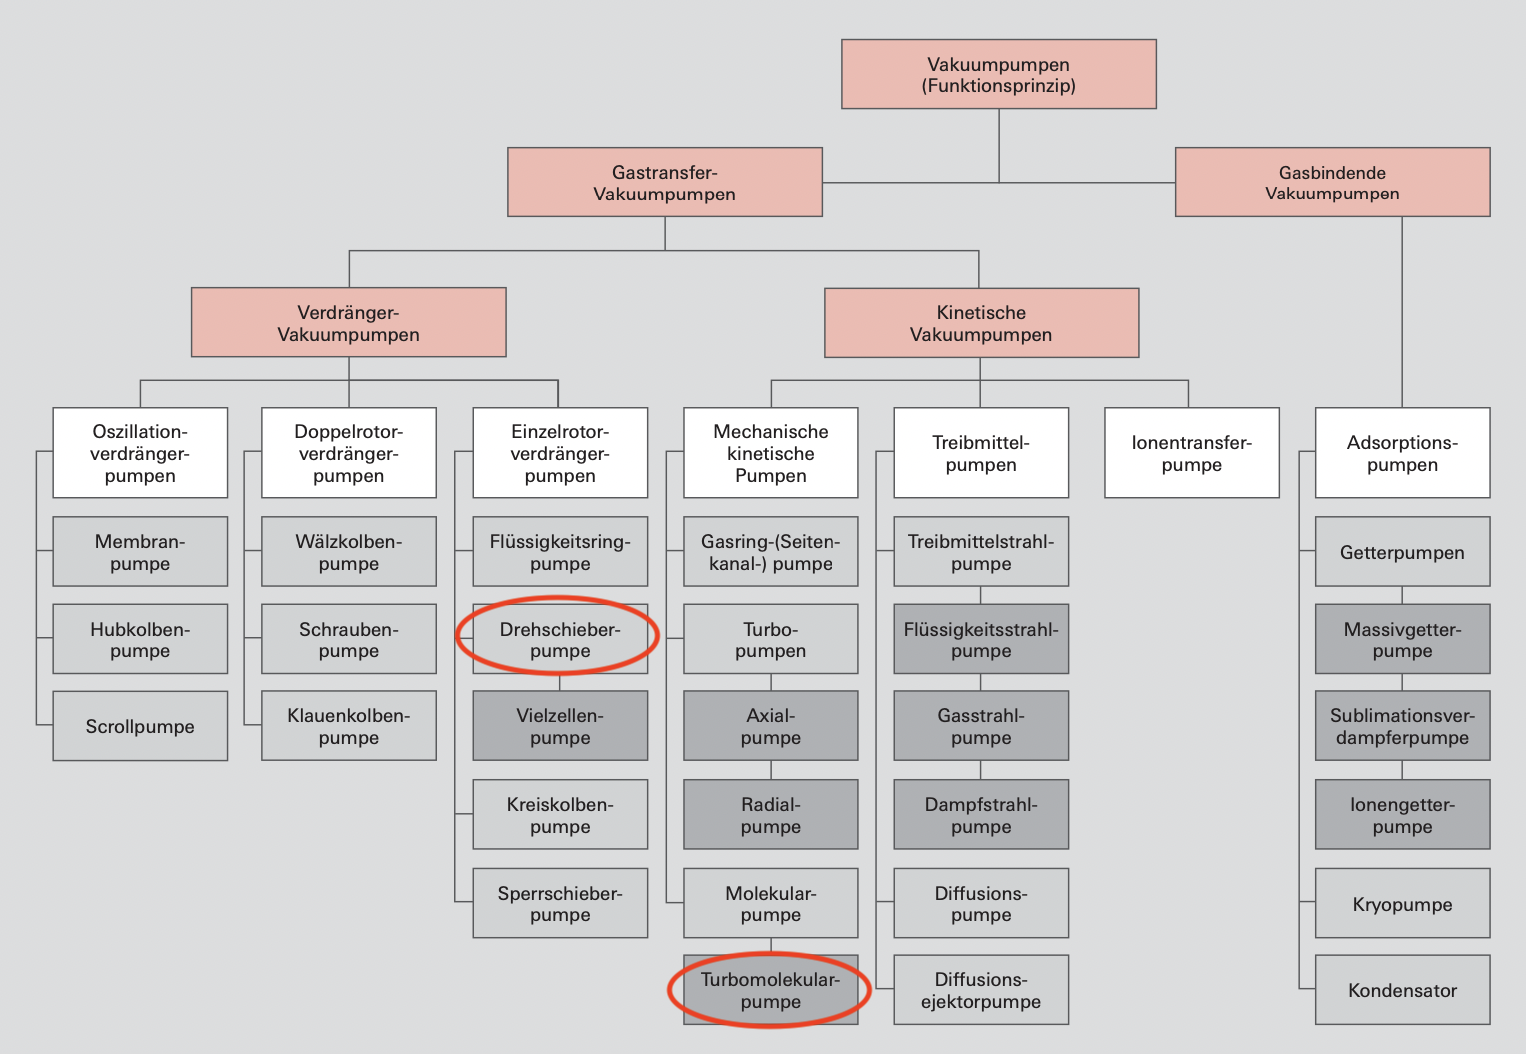
\includegraphics[width=0.9\textwidth]{abb/pumpen.png}
    \caption{Übersicht Vakuumpumpen\cite{Pfeifer}} 
    \label{fig:pumpen}
\end{figure} 
Dabei liegt der Fokus in diesem Versuch auf der Drehschieberpumpe und der Turbomolekularpumpe (rot markiert).
Beide Pumpen arbeiten in einem anderen Druck Bereich (vgl. Abb. \ref{fig:Vakuum}), 
sodass die Drehschieberpumpe der Turbomolekularpumpe vorangestellt werden muss (vgl. Kapitel \ref{sec:Durchführung}).
Klassifiziert werden die Pumpen neben ihrem Funktionsprinzip durch ihr \textit{Saugvermögen}, ihre
\textit{Saugleistung} und ihrem \textit{Enddruck}.

\subsubsection{Enddruck}
Der Enddruck ist der niedrigste Druck, den eine Pumpe theoretisch erreichen kann.
Sie nährt sich ihm asymptotisch und kann ihn niemals ganz erreichen,
da nahe des Enddruckes die Saugleistung null beträgt.
In diesem Bereich arbeitet die Pumpe ausschließlich gegen ihren Rücklaufstrom.

\subsubsection{Drehschiebervakuumpumpe}
\begin{figure}[h]
    \centering
    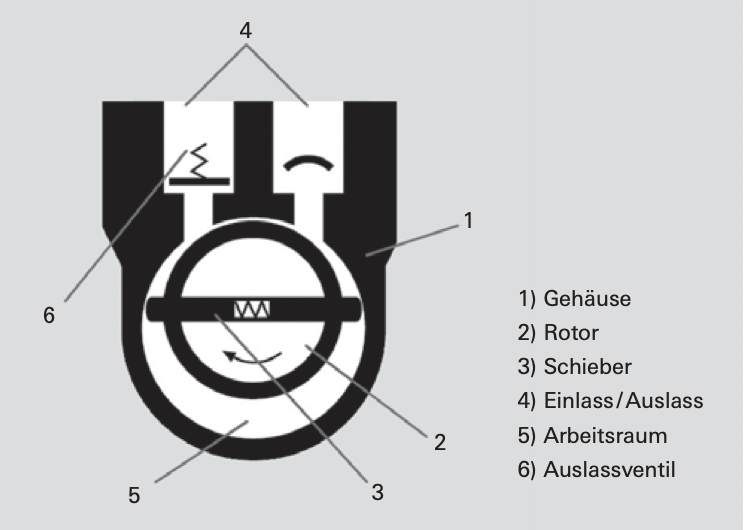
\includegraphics[width=0.5\textwidth]{abb/drehpumpe.png}
    \caption{Aufbau einer Drehschieberpumpe \cite{Pfeifer}} 
    \label{fig:drehpumpe}
\end{figure} 
Die Drehschieberpumpe besteht aus einem asymmetrisch eingesetzten Schieber, 
welcher sich dreht und dadurch das Gas vom Einlassventil zum Auslassventil transportiert.
Abgedichtet wird der Aufbau durch eine dünne Ölschicht an den Innenwänden.
Die Funktionsweise lässt sich gut durch die ideale Gasgleichung verstehen \eqref{eq:idealgaß}.
Der Schieber entspannt zuerst das Gas, 
wodurch der Druck abnimmt (bei konstanter Temperatur).
Beim Auslassventil findet der inverse Prozess statt.
Das Gas wird komprimiert, wodurch der Druck steigt 
und das Medium aus dem Ventil gedrückt wird.

Die Drehschieberpumpe kann nur einen vergleichsweise hohen Enddruck erreichen,
da der Ölfilm nur begrenzt dichthält.
Gleichzeitig gelangt auch immer ein kleiner Ölanteil in den Rezipienten.
\newpage
\subsubsection{Turbomolekularpumpe}
Die Turbomolekularpumpe ist ähnlich einer Turbine aufgebaut.
\begin{figure}[h]
    \centering
    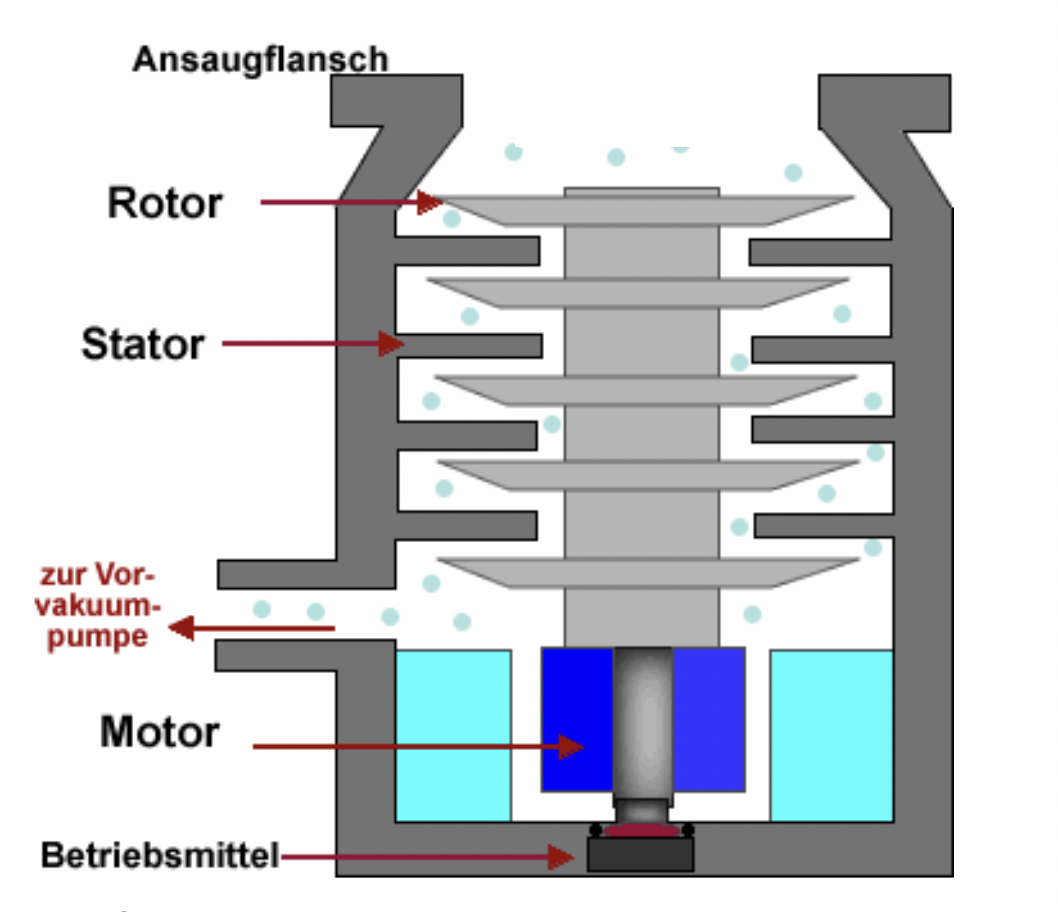
\includegraphics[width=0.5\textwidth]{abb/Turbopumpe.png}
    \caption{Skizzenhafter Aufbau einer Turbomolekularpumpe \cite{turbo}}
    \label{fig:turbo}
\end{figure}
Sie besteht aus einem sich schnell drehendem Rotor und einem Stator (vgl. Abb. \ref{fig:turbo}).
Das zugrundeliegende Funktionsprinzip ist die Impulsübertragung.
Die Rotorblätter absorbieren die Gasmoleküle, 
wenn diese die Rotorblätter wieder verlassen, besitzen sie zusätzlich zu ihrer thermischen Geschwindigkeit den Impuls des Rotors.
Damit die zusätzliche Geschwindigkeit nicht durch Kollisionen unter den Gasteilchen verloren geht,
muss die mittlere freie Weglänge größer sein als der Schaufelabstand.
Dies ist nur bei der molekularen Strömung der Fall.
Daher benötigt die Turbomolekularpumpe eine Vorvakuumpumpe,
welche den Druck entsprechend weit reduziert.

Der Vorteil der Turbomolekularpumpe gegenüber der Drehschieberpumpe ist,
dass sie ohne Öl auskommt.
Dadurch sind wesentlich niedrigere Enddrücke zu erreichen.


\subsection{Saugvermögen}
Das Saugvermögen ist gegeben durch 
\begin{equation}
    S =\frac{\text{d}V}{\text{d}t}
\end{equation}
Sie gibt den mittlere Volumenstrom an,
der durch die Ansaugöffnung der Vakuumpumpe pro Zeit durchgesetzt wird.

Die Saugleistung gibt das Saugvermögen in Abhängigkeit vom Ansaugdruck an
\begin{equation}
    Q = S\cdot p,
    \label{eq:leckQ}
\end{equation}
da das Saugvermögen mit abnehmendem Druck ebenfalls abnimmt.

\subsubsection{Evakuierungskurve}
Für ideale Gase gilt nach Boyle mit konstanter Temperatur $T$:
\begin{equation*}
    p\cdot V = \text{const.}
\end{equation*}
Durch Ableiten nach der Zeit ergibt sich
\begin{equation*}
    S = \frac{\text{d}V}{\text{d}t} = -\frac{V}{p}\frac{\text{d}p}{\text{d}t}.
\end{equation*}
Aufgelöst nach $p(t)$ mit dem Rezipientenvolumen $V_0$ und dem Anfangsdruck $p_0$ ergibt sich unter der Berücksichtigung des Enddruckes $p_E$
\begin{equation*}
    p(t)=(p_0-p_E)\exp\left(-\frac{S}{V_0}t\right) + p_E
\end{equation*}
und damit für S:
\begin{equation}
    \ln\left(\frac{p-p_E}{p-p_0}\right) = -\frac{S}{V_0}t
    \label{eq:evacSaug}
\end{equation}

\subsubsection{Leckratenmessung}
Das manuelle Einstellen eines künstlichen Lecks erbringt einen Gleichgewichtsdruck $p_g$, wenn die Pumpe genauso viel Gas absaugen kann wie in den Rezipienten reinströmt.
In diesem Zustand gilt nach \autoref{eq:leckQ} bei Abschalten der Pumpe
\begin{equation*}
    S = \frac{Q}{p_g}
\end{equation*}
mit der Leckrate
\begin{equation*}
    Q = V_0 \cdot\frac{\text{d}p}{\text{d}t}
\end{equation*}
und somit
\begin{equation}
    S = \frac{V_0}{p_g}\cdot\frac{\text{d}p}{\text{d}t}.
    \label{eq:leckSaug}
\end{equation}



\subsection{Druckmessung}
Der Druck ist definiert als Kraft pro Fläche.
Dadurch lässt er sich direkt durch die Kraft, 
welche auf eine Membran wirkt, messen.
Die Messung der Auslenkung erfolgt beispielweise durch einen Piezokristall.
Nimmt der gemessene Druck allerdings stark ab,
ist die auf die Membran wirkende Kraft irgendwann so klein, 
dass keine Auslenkung mehr gemessen werden kann.
Der Druck muss ab diesen Punkt indirekt gemessen werden.
Dies kann durch den Zusammenhang zwischen Druck und Wärmeleitfähigkeit
oder auch durch die Beobachtung der Ionisationsströme geschehen.

\subsubsection{Pirani-Vakuummeter}
In einem gewissen Druckbereich (vgl. Abb. \ref{fig:wärme}) ist die Wärmeleitfähigkeit linear abhängig vom Druck.
\begin{figure}[h]
    \centering
    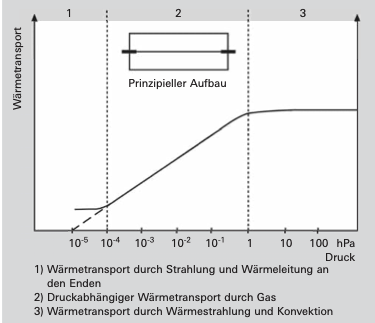
\includegraphics[width=0.5\textwidth]{abb/waerme.png}
    \caption{Zusammenhang zwischen Wärmeleitfähigkeit und Druck \cite{Pfeifer}}
    \label{fig:wärme}
\end{figure}
In diesem Bereich kann der Druck mithilfe eines Pirani-Vakuummeter gemessen werden.
Im Zentrum des Messgerätes wird ein Draht auf eine konstante Temperatur geheizt.
Durch das umgebene Gas wird die Wärme an eine Rohrwand übertragen.
Die dort gemessene Temperatur gibt Aufschluss über den Druck.
Zu beachten ist das jedes Gas eine eigene Kennlinie besitzt,
auf die das Messgerät eingestellt werden muss.

\subsubsection{Kalt-/Heißkathode Ionisationvakuummeter}
Ionisationsvakuummeter bestehen aus einer Kathode und einer Anode,
welche in einem Magnetfeld eingelassen sind.
An der Kathode werden nun Elektronen emittiert,
hierbei unterscheiden sich Kalt- und Heißkathode.
Bei der Heißkathode geschieht dies durch den glühelektrischen Effekt,
bei der Kaltkathode durch eine angelegte Spannung.
Die emittierten Elektronen fliegen
durch die Lorentzkraft auf Kreisbahnen gezwungen
Richtung Anode.
Dabei Ionisieren sie die sich im Aufbau befindenden Gasteilchen.
Der dadurch gemessene Ionisationsstrom ist proportional zum Druck.
Die Kreisbahn ist dafür notwendig,
um die Wahrscheinlichkeit zu erhöhen, ein Gasmolekül zu ionisieren. 
